\section{Database access models}

\begin{frame}
  \frametitle{Databases}
  \begin{example}[Typical relational database in a tax office]
  \begin{tabular}{l|l|l|l|l|l|l}
    ID & Name &  Salary & Deposits & Age & Postcode & Profession\\
    \hline
    1959060783 & Mike Pence & 150,000 & 1e6 & 60 & 1001 & Politician\\
    1946061408 & Donald Trump & 300,000 & -1e9 & 72 & 1001 & Rentier\\
    2100010101 & A. B. Student & 10,000 & 100,000 & 40 & 1001 & Time Traveller
  \end{tabular}
\end{example}

\only<1>{
  \begin{block}{Database access}
    \begin{itemize}
    \item When owning the database: Direct look-up.
    \item When accessing a server etc: Query model.
    \end{itemize}
  \end{block}
}
\only<2>{
  \begin{figure}[H]
    \centering
    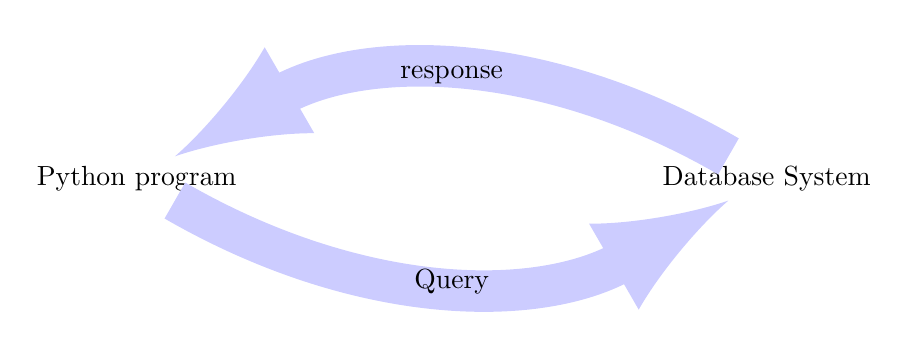
\begin{tikzpicture}
        \node[rectangle] at (0,0) (python) {Python program};
        \node[rectangle] at (8,0) (database) {Database System};
        \draw[->, >=latex, blue!20!white, line width=15pt, bend right]   (python) to node[black]{Query} (database) ;
        \draw[->, >=latex, blue!20!white, line width=15pt, bend right]   (database) to node[black]{response} (python) ;
      \end{tikzpicture}
    \label{fig:database-access}
    \caption{Database access model}
  \end{figure}
}
  
\end{frame}

\begin{frame}
  \frametitle{Queries in SQL}
  \begin{block}{The \texttt{SELECT} statement}
    \begin{itemize}
    \item \texttt{SELECT column1, column2 FROM table;}
      \only<article>{This selects only some columns from the table}
    \item \texttt{SELECT * FROM table;}
      \only<article>{This selects all the columns from the table}
    \end{itemize}
  \end{block}

  \begin{block}{Selecting rows}
    \texttt{SELECT * FROM table WHERE column = value;}
  \end{block}

  \begin{exampleblock}{Arithmetic queries}
    \only<article>{Here are some example SQL statements}
    \begin{itemize}
    \item  \texttt{SELECT COUNT(column) FROM table WHERE condition;}
      \only<article>{This allows you to count the number of rows matching \texttt{condition}}
    \item  \texttt{SELECT AVG(column) FROM table WHERE condition;}
      \only<article>{This lets you to count the number of rows matching \texttt{condition}}
    \item  \texttt{SELECT SUM(column) FROM table WHERE condition;}
      \only<article>{This is used to sum up the values in a column.}
    \end{itemize}
  \end{exampleblock}

\end{frame}



%%% Local Variables:
%%% mode: latex
%%% TeX-master: "notes"
%%% End:
